% Wall-lattice fluctuations, mobility and pinning (2026-10-06). Scripts: theory/fluct/
\subsection{Fluctuations, mobility and pinning of the wall lattice}\label{sec:fluct}
\emph{Question (B.~Loewe):} perturb the elastic energy of the wall defects about their equilibrium, add the hydrodynamic forcing, and check the stability
of the layer; on the way, find how much wall defects wander, and use that to build imperfect lattices for the one-vortex/two-vortex question
(Sec.~\ref{sec:hydro}). This subsection collects the passive part (stage~1), the defect mobility, the origin of the pinning, the measured active
wandering, and the imperfect-lattice test (stage~2).

\paragraph{Stage 1: harmonic theory.} Expanding the energy of Eq.~\eqref{eq:Eel} to second order about the relaxed ring (circle) or the relaxed
lattice (ellipse, conformal map), with Hessian $\mathsf H$ in units of $\pi K$, equipartition gives $\langle\delta x\,\delta x^T\rangle=(k_BT/\pi K)\,\mathsf H^{+}$,
projected on the local wall tangent and normal. There is no free parameter once $K$ is fixed. Measurement: passive runs, wall $+\half$ tracked
frame to frame (cyclic relabelling), displacements about each site's mean; ``internal'' removes the collective sliding
(\texttt{theory/fluct/measure\_passive.py}, \texttt{fluct\_theory.wl}).
\begin{itemize}
  \item \textbf{Along the wall the $N$-dependence is exact up to one constant.} Measured/predicted rms with $K=32.5\,k_BT$ (mean of $K_1$, $K_3$) is
        $1.35\pm4\%$ in every case: circles $N=4$--20 ($R=31.83$), $R=27.28$, and passive ellipses $\varepsilon=1.2$, 1.5, 2.0 (Fig.~\ref{fig:fluct}).
        A harmonic fit would give $K_\mathrm{eff}=17.8\,k_BT$.
  \item \textbf{Sliding is a zero mode of the one-constant theory.} A rigid rotation of the ring costs nothing in a circle. In ellipses the sliding
        eigenvalue is $10^{-7}$, $8\times10^{-6}$ and $10^{-4}$ (internal modes from $4\times10^{-3}$), i.e.\ a predicted sliding rms of 84, 10 and
        2.7 cells at $\varepsilon=1.2$, 1.5, 2.0. Measured: 0.3--1 cell in circles and ellipses alike. Something outside the one-constant theory pins
        the lattice (below).
\end{itemize}
\begin{figure}[H]\centering
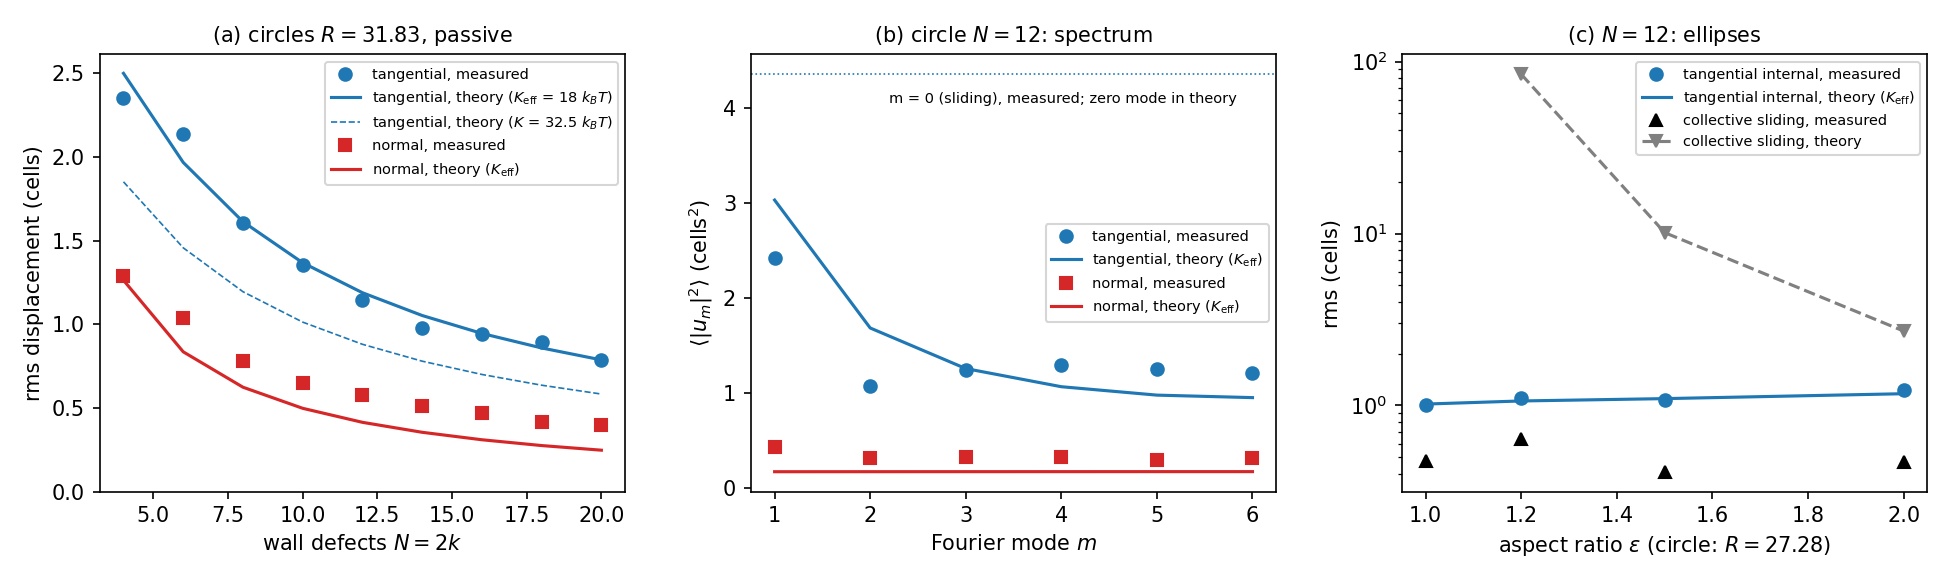
\includegraphics[width=\textwidth]{fluct.png}
\caption{Passive wall-lattice fluctuations, harmonic theory vs measurement. (a) Circles $R=31.83$: rms tangential (internal) and normal displacement
against $N=2k$; dashed: theory with $K=32.5\,k_BT$; solid: with the single fitted $K_\mathrm{eff}=17.8\,k_BT$. (b) Circle $N=12$: spectrum of the
tangential and normal displacements per Fourier mode $m$; dotted: measured $m=0$ (sliding), a zero mode of the theory. (c) $N=12$ ellipses: internal
tangential rms (theory with $K_\mathrm{eff}$) and collective sliding rms, measured (0.4--0.6 cells) and predicted by the one-constant theory (log scale).}\label{fig:fluct}
\end{figure}

\paragraph{Exact potential and the detector.} The harmonic expansion and the raw positions both hide something. (i) The image repulsion is steep
towards the wall and soft towards the bulk. (ii) Both defect trackers (default union-find and legacy, \texttt{pout.c}) write the centre of mass of the cluster of
cells flagged as the core (cell centres at $i+\tfrac12$); the usual cluster is a $2\times2$ block around a cell corner, so 93--98\% of the coordinates are integers and the
rest multiples of $\tfrac16$ or $\tfrac12$ (same in both trackers). The positions are thus quantised to the cell grid, which adds about $1/\sqrt{12}\approx0.29$ cells per
coordinate. Exact Boltzmann sampling (Metropolis) of the full disk energy, with the wall
offset of 0.61 cells from Fig.~\ref{fig:depthlaw} and the sampled positions rounded to the grid like the detector (\texttt{mc\_exact.py},
Fig.~\ref{fig:fluctmc}):
\begin{itemize}
  \item \textbf{Along the wall, $K=K_3=23\,k_BT$ (the measured bend constant) reproduces the data within 2--4\%} for $N=8$--20 (and the mean depth
        within 0.05 cells). The ``$K_\mathrm{eff}$'' of the harmonic fit was mostly detector rounding and mild anharmonicity: tangential displacements of
        wall $+\half$ cost bend.
  \item \textbf{Across the wall a residual remains}, growing for deeper layers: in quadrature $\approx0.15$ cells ($N=20$), 0.35 ($N=12$) and 0.5
        ($N=4$--8). This residual is the target of the random-walk test below.
\end{itemize}
\begin{figure}[H]\centering
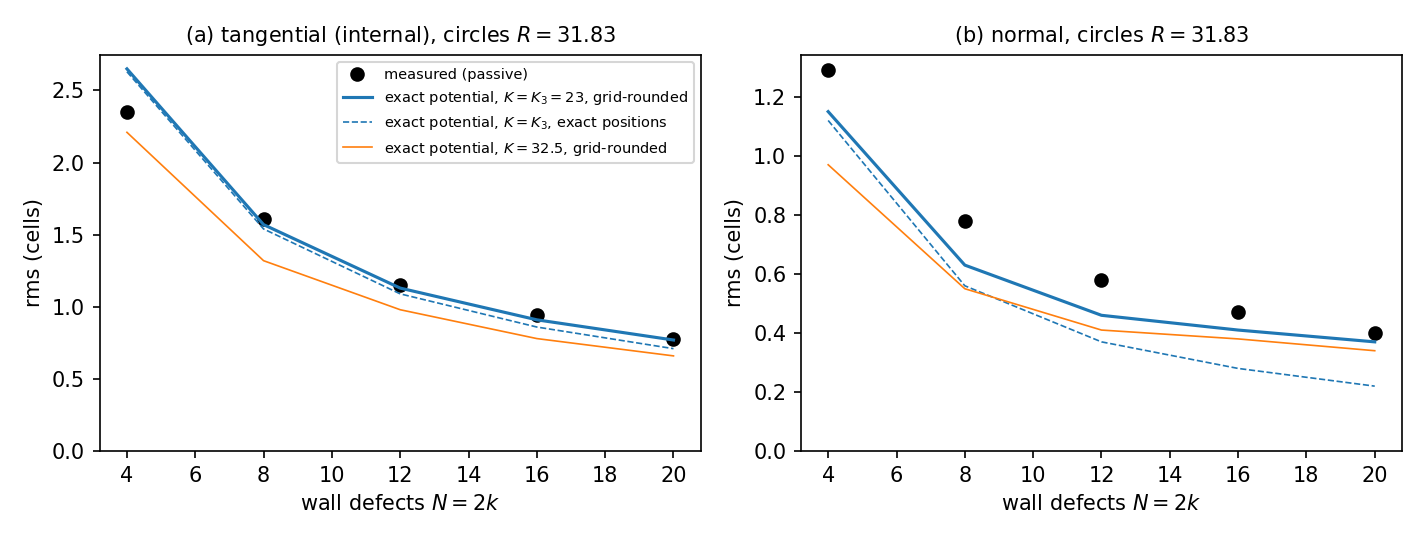
\includegraphics[width=0.85\textwidth]{fluct_mc.png}
\caption{Passive circles $R=31.83$: measured rms displacement (a) along and (b) across the wall against exact Monte Carlo of the full electrostatic
energy (wall offset 0.61). Solid blue: $K=K_3=23\,k_BT$ with positions rounded to the cell grid as in the detector; dashed: exact positions;
orange: $K=32.5\,k_BT$, rounded.}\label{fig:fluctmc}
\end{figure}

\paragraph{Random walks with fluid noise (B.~Loewe's test).} Overdamped Langevin dynamics of the $2k$ wall $+\half$ in the full potential
($K=K_3$, wall offset 0.61, $\mu=0.03$), with white thermal noise plus advection by the cavity fluid: an Ornstein--Uhlenbeck velocity per defect,
tangential and normal, with the variance and correlation time measured at the defect depth in a dedicated passive run
(\texttt{runs/fluidnoise/passive\_R27\_k06}, instantaneous cell velocities every time unit, smoothed over 1.5 cells): rms 0.042--0.049 cells per
time unit, correlation time 0.9--2.6 (shorter near the wall), the same along and across the wall (\texttt{langevin/}). Positions rounded as in
the detector.
\begin{table}[H]\centering\small
\caption{Random walks of the passive wall lattice ($R=31.83$): rms along/across the wall (cells) and median relaxation time of the internal modes.
Fluid noise $\times\lambda$: the measured fluid velocity noise scaled by $\lambda$.}\label{tab:langevin}
\begin{tabular}{lccc}\toprule
& $N=4$ & $N=12$ & $N=20$\\\midrule
measured & 2.35 / 1.29 & 1.15 / 0.58 (37) & 0.78 / 0.40 (12)\\
thermal only & 2.67 / 1.16 & 1.14 / 0.47 (21) & 0.77 / 0.37 (8)\\
thermal + fluid $\times1$ & 2.87 / 1.22 & 1.19 / 0.48 (23) & 0.80 / 0.38 (8)\\
thermal + fluid $\times2$ & 3.34 / 1.43 & 1.36 / 0.52 (23) & 0.89 / 0.39 (8)\\
thermal + fluid $\times4$ & 4.78 / 2.19 & 1.89 / 0.70 (22) & 1.19 / 0.44 (9)\\
fluid only $\times1$ & 1.00 / 0.51 & 0.49 / 0.29 (20) & 0.35 / 0.23 (11)\\\bottomrule
\end{tabular}
\end{table}
\begin{itemize}
  \item At its measured strength the fluid noise adds only 2--5\% to the spreads: its effective diffusivity
        $\langle u^2\rangle\tau\approx0.003$ is a tenth of the thermal $\mu k_BT$. Alone it gives far too little.
  \item Closing the normal gap at $N=12$ would need $\lambda\approx3$, which already overshoots the tangential spread (1.36--1.89 against 1.15).
        The normal excess is therefore not extra isotropic noise: it is specific to the direction across the wall, most likely the detector near the wall
        (the core is distorted by the wall, so its located centre jitters more across than along it), beyond the grid rounding already included.
  \item The relaxation times of the internal modes come out 1.5--1.8$\times$ shorter than measured with $\mu=0.03$, i.e.\ $\mu\approx0.02$ once the
        variances are not inflated by the detector (the model-free estimate below uses the measured, rounding-inflated variances).
\end{itemize}

\paragraph{Mobility.} Overdamped relaxation of mode $m$ with stiffness $k_m=k_BT/\langle|u_m|^2\rangle$ gives
$\mu=\Gamma_m\langle|u_m|^2\rangle/k_BT$, with $\Gamma_m$ the inverse $1/e$ time of the mode autocorrelation. This is model-free: it uses only
measured variances and times (\texttt{mobility.py}). Passive circles $N=8$--20: $\mu\approx0.03$ cells$^2/(k_BT\,\tau)$ (median per run
0.025--0.048), so $D=\mu k_BT\approx0.03$ cells$^2/\tau$. Internal modes relax in 10--40 time units, $m=1$ in 40--230.

\paragraph{The pinning is not the grid.} The MPCD collision grid is randomly shifted every step (\texttt{galInv} = 1), so a fixed-grid pin could
enter only through the detector, and would have a period of about one cell, i.e.\ a random registry in every run. Instead the registry of the wall
lattice with the anchoring pattern is reproducible:
\begin{itemize}
  \item Active circles (all densities and seeds, $k=2$--10): $Z=\langle N_w^{-1}\sum_je^{i(2k-2)\phi_j}\rangle$ has the same phase in different runs,
        mean resultant length 0.43--0.64 against $\approx0.2$ for random phases (e.g.\ $k=6$: 31 runs, Rayleigh $p\approx10^{-4}$), mean phase within
        $\pm0.26$ rad of 0 for every $k$.
  \item Passive circles ($R=13$--64): the phase of $Z_{2k}$ agrees across radii, resultant length 0.65--0.97 against $\approx0.3$. \textbf{But this is
        inherited from the common initial condition} (all production runs start with the director along $y$, \texttt{oDist}=2): eight passive runs
        ($k=6$, $R=31.83$) started along $x$, at $45^\circ$, along $y$ (new seeds) and random settle at different registries, arg $Z$ = $-2.62$ ($x$), $-1.44$
        ($45^\circ$), $-0.07$, $-0.23$, $+0.69$ ($y$), $+0.01$, $+1.20$, $+0.48$ (random), roughly $2(\beta_0-90^\circ)$ for an initial angle $\beta_0$, and only
        creep (0.3--0.5 rad over 3000 time units; Rayleigh $p\approx0.1$ across runs; \texttt{runs/pinning\_ic}, \texttt{ic\_test.py}). The passive registry is
        a symmetry broken by the initial condition and then frozen (B.~Loewe's hypothesis), consistent with a first-order anisotropy barrier below
        $1\,k_BT$ for the incommensurate passive ring. One random start trapped an extra $\pm\half$ pair.
  \item \textbf{The active registry is pinned, independent of the initial condition.} Six active runs ($k=6$, $R=31.83$, $\zeta=0.07$) started random
        ($\times3$), along $x$, at $45^\circ$ and along $y$, plus two production seeds: every run ends at arg $Z=+1.17$ or $-1.17$ rad (concentration 1.00 within
        each run, no creep), i.e.\ at $\pm\tau$ with the measured tilt $\tau=63$--$64^\circ$, one value per circulation sense. Corrected by the lock,
        $D=\arg Z-\tau=+0.03\pm0.07$ in all eight (resultant length 1.00, Rayleigh $p\approx3\times10^{-4}$): the predicted site, whatever the start. Only the
        chirality (sense of rotation) is chosen spontaneously (\texttt{runs/pinning\_ic\_active}, \texttt{ic\_test\_active.py}).
\end{itemize}

\paragraph{Tilt and position are locked.} The anchoring director $\psi=k\phi$ is invariant only under rotations by $2\pi/(2k-2)$. In the one-constant
solution (defects plus same-sign images) a rigid rotation $\alpha$ of the lattice costs nothing but tilts every $+\half$ head, relative to its wall
normal, by $(2k-2)\alpha$; for a defect at the wall, $\text{tilt}_j=(2k-2)\phi_j+\text{const}$. Tests (\texttt{pinning/}):
\begin{itemize}
  \item \textbf{Passive:} the collective tilt follows the collective rotation with slope $0.87$--$0.92\times(2k-2)$, correlation 0.95--0.97
        ($k\ge5$). Along a $2k$ ring the mean tilt steps by $-2\cdot2\pi/N$ per defect ($k=6$: $+41^\circ,-20^\circ,-91^\circ,\dots$), as predicted:
        the passive heads do not all point at the wall.
  \item \textbf{Active ($N=2k-2$, $\approx$150\,000 frames, $k=3$--10):} $D=\arg Z-\bar\tau$ (registry minus mean tilt) is the same in every frame of
        every run, resultant length 0.99, mean 0.00; within runs $\arg Z$ follows $\bar\tau$ with slope 1.04--1.15 (theory 1).
\end{itemize}
So the $2k-2$ sites are the positions where the recorded angle (the tail, $\nabla\!\cdot Q$) points straight at the wall, i.e.\ the head points straight into the bulk, and a wall defect cannot tilt without sliding off its site:
the coherent $63^\circ$ tilt of the active circles shifts the lattice by $63^\circ/(2k-2)$ ($k=6$: 3.5 cells at $R=32$).

\paragraph{What pins the registry: splay $\neq$ bend.} With $K_{1,3}=K\pm\Delta$ the first-order correction to the energy is
$\Delta F=\frac{\Delta}{2}\int(\text{splay}^2-\text{bend}^2)\,dA$ on the exact one-constant field, which depends on the registry. Integrated
numerically with a smooth core cutoff $a$ (\texttt{anisotropy\_pinning.py}; $K_1=42.0$, $K_3=23.1$, $\Delta=9.45\,k_BT$; Fig.~\ref{fig:anisopin}):
\begin{itemize}
  \item \textbf{Active ring} ($2k-2$ wall $+\half$ and a central $+1$): the minimum is exactly at zero tilt (heads at the wall), the measured
        registry. The barrier is 80--110\,$k_BT$ ($k=6$), 45--70 ($k=8$), 100--170 ($k=4$). The curvature predicts a collective rms of 0.45--0.51 cells
        ($k=6$, $R=31.8$, $a=0.5$--2), against 0.29--0.36 measured in the pinned active circles at that radius: the right order and the right site,
        with no free parameter.
  \item \textbf{Passive ring} ($2k$ defects, incommensurate with the $2k-2$-fold pattern): the first-order barrier is only 0.1--1\,$k_BT$ and depends on
        the core cutoff, consistent with the initial-condition test: the passive registry is not pinned but frozen in from the start, its slow creep
        set by the small collective mobility.
  \item In a one-constant model (such as the Q-tensor model of Norton \emph{et al.}) this pinning would be absent: the sliding of the wall lattice
        would be free.
\end{itemize}
\begin{figure}[H]\centering
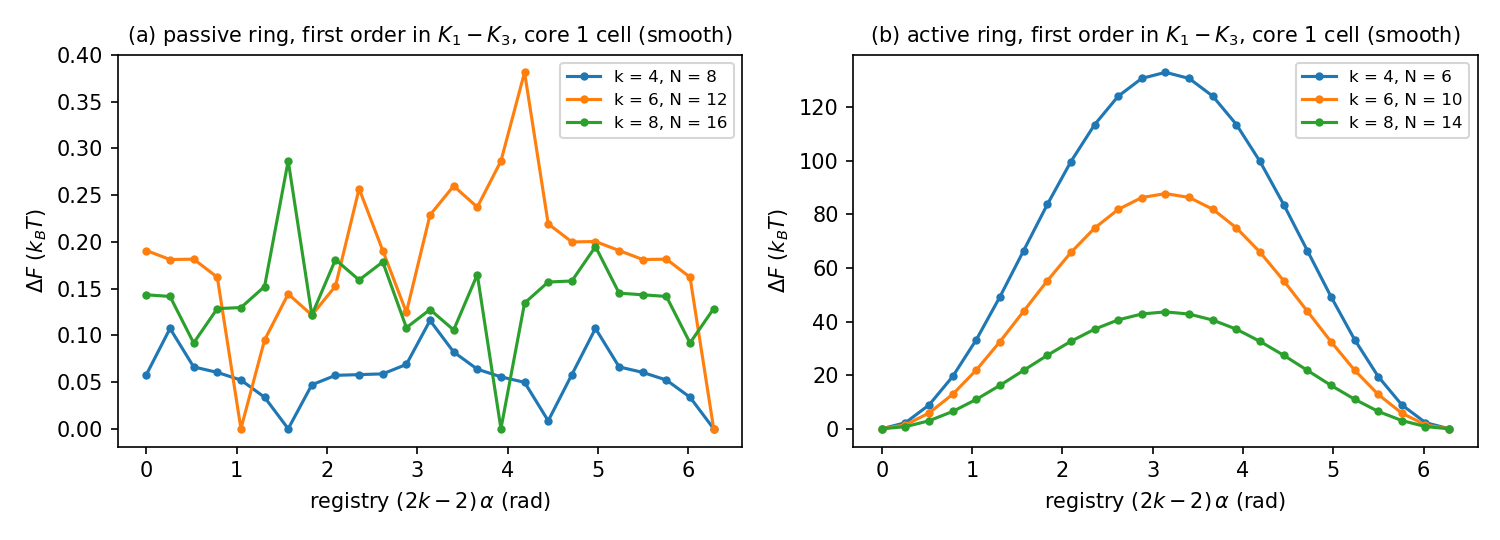
\includegraphics[width=0.9\textwidth]{anisotropy_pinning.png}
\caption{Registry potential of the wall lattice from splay--bend anisotropy (first order in $K_1-K_3$, smooth core cutoff of 1 cell), against
the registry $(2k-2)\alpha$; zero = heads pointing at the wall. (a) Passive ring of $2k$: below $1\,k_BT$. (b) Active ring of $2k-2$ with a
central $+1$: barriers of tens of $k_BT$, minimum at zero tilt.}\label{fig:anisopin}
\end{figure}

\paragraph{How much wall defects wander in active runs.} Disorder is measured as $\sigma_\mathrm{gap}=\mathrm{sd}(g)/\sqrt2$, with $g$ the
arclength gaps between neighbouring wall $+\half$. For independent Gaussian displacements about evenly spaced sites this is exactly $\sigma_t$, the
disorder parameter of the stage-2 ensembles, and needs no tracking (passive check: $\sigma_\mathrm{gap}=1.03$--1.17 against tracked 1.01--1.23;
\texttt{active\_wander.py}, Fig.~\ref{fig:wander}).
\begin{itemize}
  \item \textbf{Active circles} ($k=6$, $R/\ell_a=0.4$--2.2): $\sigma_\mathrm{gap}=0.6$--1.5 cells, the passive level; the wall count is $2k-2=10$ in
        75--93\% of frames. At $R/\ell_a=2.9$ the lattice melts ($\sigma_\mathrm{gap}\approx9$, count $7.6\pm2.2$).
  \item \textbf{Active ellipses:} $\varepsilon=1.2$: $\sigma_\mathrm{gap}=1.3$ (count $9.8\pm0.6$); $\varepsilon=1.5$: 6.3--6.5 (count $7.7\pm1.1$);
        $\varepsilon=2.0$: 8.1--8.4 (count $7.3\pm1.1$), both seeds. The lattice also slides freely (collective rms of tens of cells).
\end{itemize}
The realistic stage-2 disorder is therefore $\sigma_t\approx1$ for circles and $\varepsilon=1.2$, and $\sigma_t\approx6$--8 with 2--3 vacancies for
$\varepsilon=1.5$--2.
\begin{figure}[H]\centering
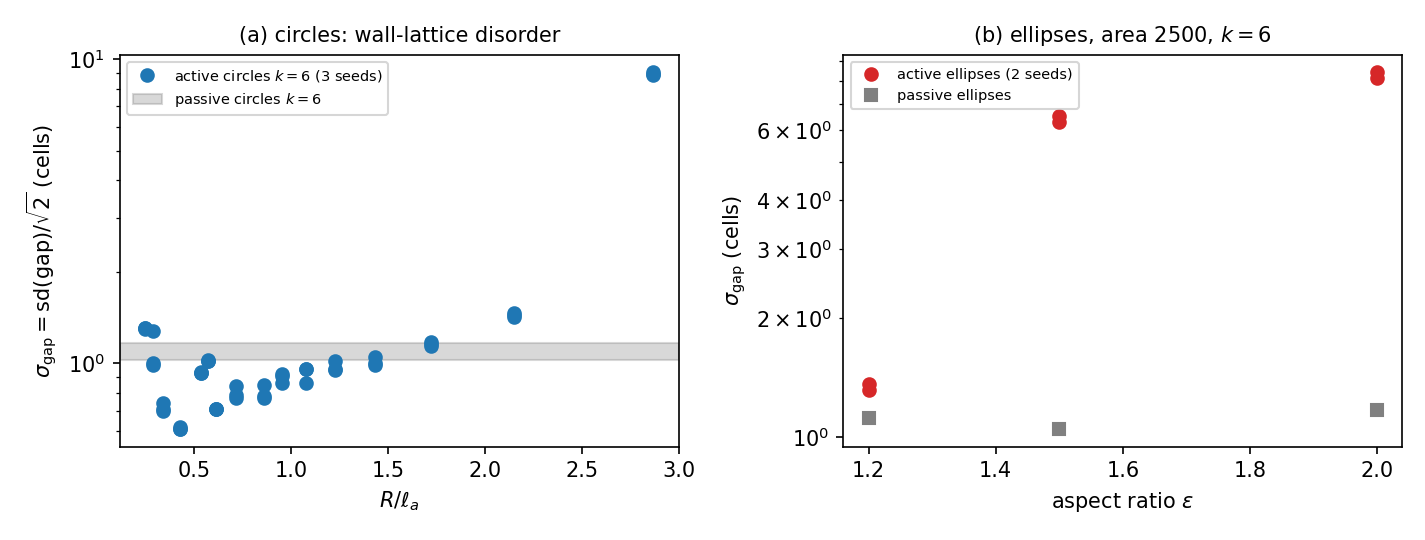
\includegraphics[width=0.9\textwidth]{active_wander.png}
\caption{Wall-lattice disorder $\sigma_\mathrm{gap}$ (log scale). (a) Active circles $k=6$, three seeds, against $R/\ell_a$; grey band: passive circles.
(b) Ellipses of area 2500, $k=6$: active (two seeds) and passive.}\label{fig:wander}
\end{figure}

\paragraph{Stage 2: imperfect lattices.} \textbf{(See the correction box in Sec.~\ref{sec:hydro}: with the physical force direction the feedback is negative, the wall layer damps
every tilt pattern and the one-vortex pattern most; the ``gain ratio'' below then measures how much more strongly one vortex is braked than two.)} For each configuration of wall $+\half$, the Stokes feedback matrix $M_{ij}$ (Sec.~\ref{sec:hydro}) is
computed and its top mode classified as one-vortex or two-vortex by its overlap with the uniform and the left/right-antisymmetric patterns
(\texttt{stage2/}). Gain ratio $=$ largest one-vortex eigenvalue / largest two-vortex eigenvalue (above 1: the layer prefers one vortex).
\begin{itemize}
  \item \textbf{Synthetic disorder (4\,845 configurations).} Lattices of 10 wall $+\half$ (area 2500, depth 1.5), tangential disorder
        $\sigma_t=0.5$--6 cells (normal 0.5), 1--3 vacancies, and the realistic active disorder ($\sigma_t=6$ or 8 with 2 or 3 vacancies), 60--80
        samples per class, $\varepsilon=1$, 1.2, 1.5, 2.0, 2.5. Up to $\varepsilon=1.5$ the top mode is one-vortex in every sample (95\% upper bound
        5--6\% per class); at $\varepsilon=2.0$ only 1/60 in the two most disordered classes. Only at $\varepsilon=2.5$ with realistic disorder does the
        two-vortex mode win in a minority of lattices: 8--15\% ($\sigma_t=6$--8, 2--3 vacancies), 2--5\% for milder disorder (Fig.~\ref{fig:stage2}).
        Disorder spreads the gain ratio but does not lower its median (1.11--1.32 everywhere, perfect lattice 1.13 in the circle, 1.05 at 2.5).
  \item \textbf{Measured wall configurations, two seeds.} One snapshot per flow interval (40 per run): top mode one-vortex in 240/240 snapshots
        ($\varepsilon=1.2$, 1.5, 2.0; seeds 1 and 2), although the measured flow has two vortices in 68--72\% ($\varepsilon=1.5$) and 48--55\%
        ($\varepsilon=2.0$) of the intervals. The gain ratio is not systematically smaller in the two-vortex intervals, and the measured tilt pattern
        barely projects on the predicted top mode (0.16--0.17 against 0.13--0.15 for a random pattern).
  \item \textbf{Reading.} Within the linear tilt-follows-flow feedback the wall layer amplifies one vortex most, whatever its disorder, up to the
        aspect ratios simulated; at $\varepsilon\approx2.5$ disorder begins to make the two-vortex state competitive. The two-vortex state of the
        $\varepsilon=1.5$--2 ellipses is imposed from outside the wall layer (the bulk), consistent with the timing in circles and with the falling wall
        share of the flow (Table~\ref{tab:hydroell}).
\end{itemize}
\begin{figure}[H]\centering
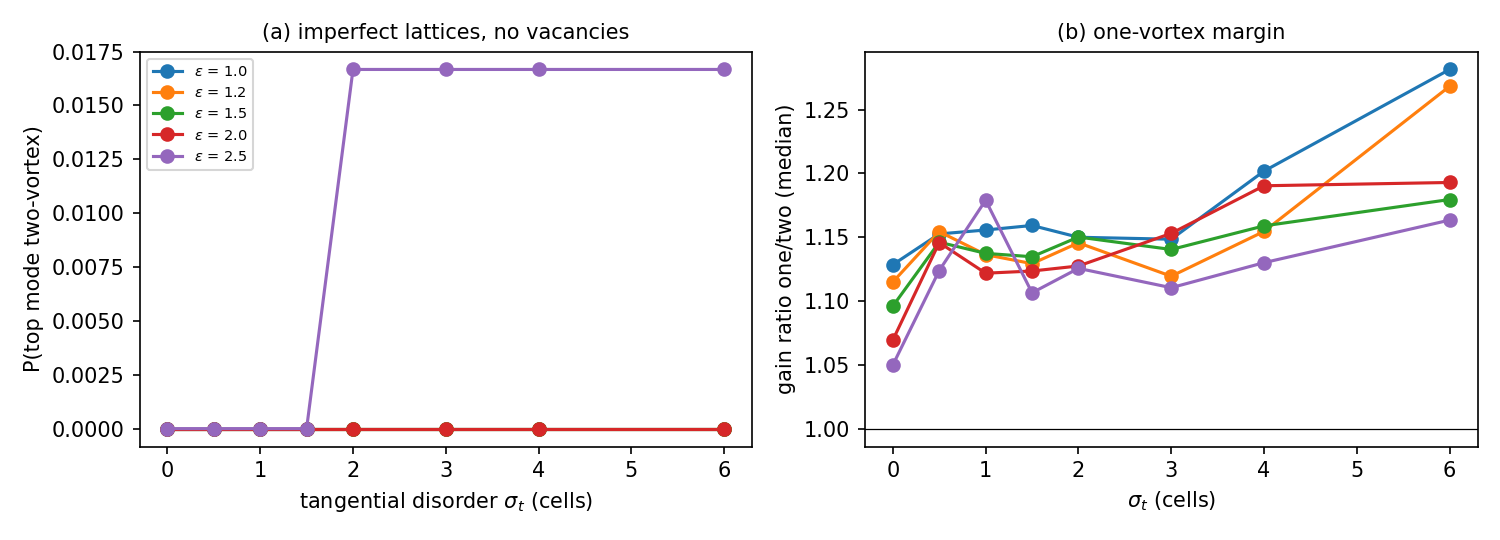
\includegraphics[width=0.9\textwidth]{stage2.png}
\caption{Stage 2. (a) Probability that the top feedback mode of a disordered wall lattice is two-vortex, against the tangential disorder
$\sigma_t$, per aspect ratio (no vacancies). (b) Median gain ratio one-vortex/two-vortex (1: degenerate).}\label{fig:stage2}
\end{figure}

